\documentclass{article}
\usepackage{graphicx} % Required for inserting images
\usepackage[top=0.9in, bottom=1in, left=1.5in, right=1.5in]{geometry}
\usepackage[utf8]{inputenc}
\usepackage[icelandic]{babel}
\usepackage[T1]{fontenc}
\usepackage[sc]{mathpazo}
\usepackage[parfill]{parskip}
\renewcommand{\baselinestretch}{1.2}
% Tables and lists
\usepackage{booktabs,tabularx}
\usepackage{multirow}
\usepackage{enumerate}
\usepackage{adjustbox}
\usepackage{multicol}
\usepackage{xcolor}
\usepackage{algpseudocode}
\usepackage{tikz}
\usepackage{nicefrac}
\usepackage{changepage}
\usepackage{fancyvrb}
\usepackage{xlop}
\usetikzlibrary{arrows, positioning, calc, graphs}

% Math
\usepackage{amsmath, amsfonts, amssymb, amsthm}
% Graphics

\usepackage{graphicx}
\usepackage{tikz}
% Code environment
\usepackage{minted}
%\usepackage{bm}
%\usepackage{siunitx}
%\usepackage{animate}
%\usepackage{hyperref}
%\usepackage{movie15}
%\usepackage{multicol}
%\usepackage{changepage}
\title{Tölvutækni og forritun Heimadæmi 5}
\author{Ragnar Björn Ingvarsson, rbi3}
\tikzset{->, >=stealth', shorten >=1pt, node distance=2cm,thick, main node/.style={circle,draw,minimum size=3em}}


\begin{document}
\renewcommand\thepage{}
	
	\maketitle

	\newpage
	\setcounter{page}{1}
	\renewcommand\thepage{\arabic{page}}

	\section{}
	\begin{itemize}
		\item[a)] 
			\begin{itemize}
				\item[i.] \textbf{EF}
				\item[ii.] \textbf{CDEF}
				\item[iii.] \textbf{0123}
				\item[iv.] \textbf{01234567}
			\end{itemize}
		\item[b)]
			\begin{itemize}
				\item[i.] \textbf{01}
				\item[ii.] \textbf{0123}
				\item[iii.] \textbf{CDEF}
				\item[iv.] \textbf{89ABCDEF}
			\end{itemize}
	\end{itemize}

	\section{}
	\begin{itemize}
		\item[a)] Við sjáum að við keyrslu fæst þetta
			\begin{center}
				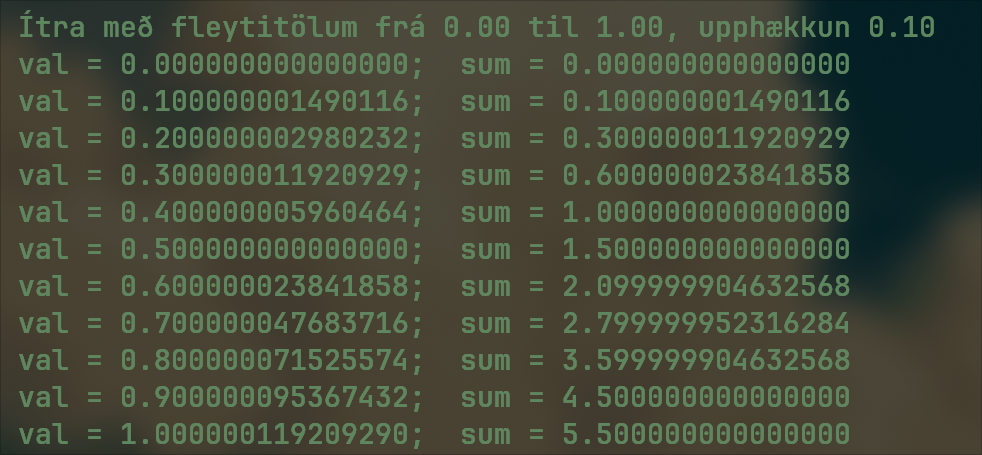
\includegraphics[scale=0.35]{floatloop.png}
			\end{center}

			En forritið átti að stoppa í $1.0$.

			Vandamálið hér er að í for lykkjunni er athugað hvort núverandi 
			gildi sé \textbf{jafnt} og $1.0$ en með fleytitölum fáum við 
			ekki svoleiðis nákvæmni. Við sjáum af myndinni að þegar val er 
			rúmlega $1.0$ er það í raun gildið $1.000000119209290$ sem c 
			telur ekki vera jafnt og $1.0$. Fleytitalan er svona ónákvæm 
			vegna þess að hún hefur byggt upp skekkju með því að reyna að 
			sýna $0.1$, $0.2$ o.s.frv. sem geta ekki verið sýndar fullkomlega 
			með fleytitölum. Þess vegna er skilyrði for 
			lykkjunnar ennþá satt og við höldum endalaust 
			áfram.
		\item[b)] Með því að breyta í double fæst

			\begin{center}
				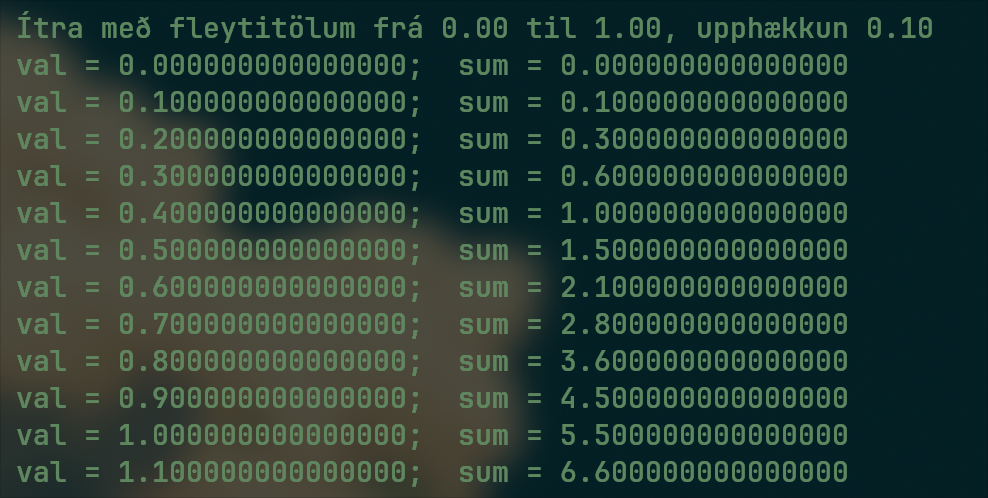
\includegraphics[scale=0.35]{double.png}
			\end{center}

			Við sjáum að með því að breyta í double höfum við vissulega 
			meiri nákvæmni en forritið heldur ennþá endalaust áfram þar sem 
			þó meiri nákvæmni sé góð, er hún ekki fullkomin, svo skekkjan 
			er ennþá til, hún er bara minni. Þess vegna helst skilyrði for 
			lykkjunnar satt og hún heldur áfram.
	\end{itemize}

	\section{}
	\begin{itemize}
		\item[a)] $1.01100$
		\item[b)] Með því að rúnna að næstu tölu viljum við fá að síðasti 
			bitinn sé $0$ en ekki $1$, semsagt slétt tala. Þess vegna 
			fáum við $1.10$, semsagt $1.5$.

			Við höfðum tvo möguleika á rúnnuninni þar sem parturinn sem við 
			vildum rúnna er mitt á milli tveggja gilda, $1.01$ og $1.10$, þ.e. 
			$1.25$ eða $1.50$. Þar sem við viljum rúnna að sléttum LSB er 
			valin $1.50$ þar sem $1.01$ endar á ás svo við veljum frekar 
			$1.10$.
	\end{itemize}

	\section{}
		Við erum semsagt með 10 bita með einn formerkisbita fremst en vitum 
		ekki hvernig skiptingin er á veldishluta og brothluta.
	\begin{itemize}
		\item[a)] Við byrjum á að breyta $3.5625$ í binary og fáum 
			$11.1001$. Síðan, þar sem IEEE vill hafa tölur á formi 
			$(-1)^{formerkisbiti}\cdot 2^{(e_me_{m-1}...e_0)_2 - 2^{m-1}-1}\cdot1.b_nb_{n-1}...b_0$ þá shiftum við tölunni um einn bitastað 
			og setjum hana fram sem $2 \cdot 1.11001$. Þá erum við komin 
			með töluna á rétt form og við sjáum að brothlutinn er að 
			lágmarki fimm bitar, $11001$.
		\item[b)] Þar sem við erum með 5 bita í brothlutann og 1 bita í 
			formerkið, þá erum við með 4 bita fyrir veldishlutann. Þá 
			fáum við að form tölunnar er $(-1)^{formerkisbiti}\cdot2^{(e_me_{m-1}...e_0)_2 - 2^{4-1}-1} 
			\cdot (1.b_nb_{n-1}...b_0)_2$. Þar sem við fáum $2 \cdot 1.11001_2$ 
			í a lið fæst:
			\[(-1)^0\cdot2^{1000_2 - 7} \cdot 1.11001_2\]
			\[= 2^{8-7} \cdot 1.11001_2\]
			\[= 2 \cdot 1.11001_2\]

			Svo talan er skilgreind svo, 0 í formerkisbita, $1000$ í 
			veldishluta og $11001$ í brothluta, eða $0100011001$ alls.
		\item[c)] Það er hægt að tákna staðlaðar tölur á þessu formi, þar 
			sem veldishlutinn getur verið samblanda af núllum og ásum.

			Hæsta staðlaða talan er þá $0111111101$ sem gefur 
			\[(-1)^0\cdot2^{11111110_2 - 127} \cdot 1.1_2\]
			\[= 2^{254 - 127} \cdot 1.5\]
			\[= 2^{127} \cdot 1.5\]
		\item[d)] Hér er ekki hægt að tákna staðlaðar tölur þar sem aðeins 
			er einn veldisbiti. Hann er annaðhvort $0$ eða $1$, sem í 
			báðum tilfellum er allur veldishlutinn sama talan, sem gerir 
			töluna ekki staðlaða.
	\end{itemize}

	\section{}

	\begin{itemize}
		\item[a)] Notum til dæmis IEEE töluna $0000010000000001_2$. Við 
			breytum henni í decimal með
			\[
				(-1)^0\cdot2^{00001_2 - 2^{5-1}-1} \cdot 
				1.0000000001_2
			\]
			\[
				= 2^{1-15}\cdot (1+2^{-10})
			\]
			\[
				= 2^{-14}\cdot (1+2^{-10})
			\]
			\[
				= 0.00006109476
			\]

			Ef við reynum svo að breyta henni í bfloat, þá sjáum við að 
			við getum haft eins veldishluta, þá $00010000$, en ekki eins 
			brothluta þar sem við erum aðeins með $7$ bita miðað við $10$ í 
			IEEE. Þá er næsta talan sem við getum fengið 
			$0000100000000000$ eða 
			\[
				(-1)^0\cdot2^{01110001_2 - 2^{8-1}-1}\cdot 1.0000000_2
			\]
			\[
				= 2^{113-127}\cdot 1
			\]
			\[
				= 2^{-14}
			\]
			\[
				= 0.00006103516
			\]
			Sem er nálægt réttu tölunni, en getur aldrei verið nógu nákvæm 
			vegna þess að bfloat er bara með minni nákvæmni.
		\item[b)] Hér viljum við þá nota styrkleika bfloat sem er stórar 
			tölur, svo við tökum töluna $0111111100000000$.

			\[
				(-1)^0\cdot2^{11111110_2 - 2^{8-1}-1}\cdot 1.0000000_2
			\]
			\[
				= 2^{254 - 127}\cdot 1
			\]
			\[
				= 2^{127}
			\]
			Hér hefur IEEE ekki roð í töluna þar sem hæsta talan sem fæst 
			úr því er $0111101111111111$.

			\[
				(-1)^0\cdot2^{11110_2 - 2^{5-1}-1}\cdot 1.1111111111_2
			\]
			\[
				= 2^{30 - 15}\cdot 1.9990234375
			\]
			\[
				= 2^{15}\cdot 1.9990234375
			\]
			\[
				= 65504
			\]
			Sem er langt frá $2^{127}$.
	\end{itemize}


\end{document}
